\chapter{Training}

\section{Datasets}


\section{Matrix Initialization}

\section{Hyperparameter Optimization}

\newpage
\section{Activation Functions}
\label{sec:activation}
\subsection{Initial \& Convolutional Layers}
At the end of each transition, an elementwise activation function is applied 
following completion of all computations.  For all but the final layer, that 
function is ReLU\footnote{NEEDS CITATION}, defined in figure \ref{fig:relu}. AS 
FOLLOWS

\begin{figure}[h]
	\centering
	\begin{minipage}{.48\textwidth}
		\begin{equation*}
			relu(x) = \begin{cases}
				0 & x < 0\\
				x & x \geq 0
			\end{cases}
		\end{equation*}
	\end{minipage}
	\begin{minipage}{.48\textwidth}
		\resizebox{\textwidth}{!}{
		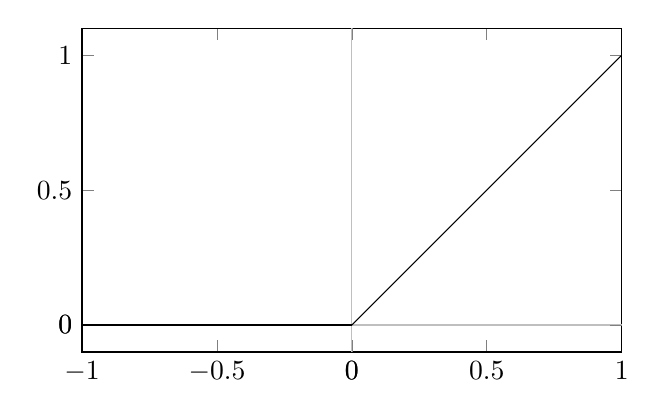
\begin{tikzpicture}
			\begin{axis}[domain=-1:1, unit vector ratio*=1 1 1,
					enlarge x limits=false, extra y ticks=0, extra x ticks=0,
					extra tick style={grid=major}]
				\addplot[color=black][domain=0:1] {x} [mark=none, smooth];
				\addplot[color=black][domain=-1:0] {0} [mark=none smooth];
			\end{axis}
		\end{tikzpicture}
		}
	\end{minipage}
	\caption{ReLU function definition and graph}
	\label{fig:relu}
\end{figure}\noindent

\subsubsection{Alternative Activations}
In addition to ReLU, we considered a sigmoid activation function:

\begin{figure}[h]
	\centering
	\begin{minipage}{.48\textwidth}
		\begin{equation*}
			S(x) = \frac{1}{1 + exp(x)}
		\end{equation*}
	\end{minipage}
	\begin{minipage}{.35\textwidth}
		\resizebox{\textwidth}{!}{
		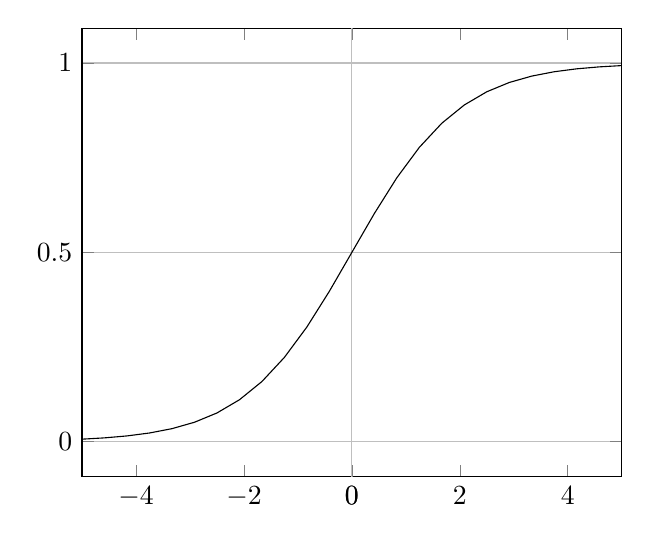
\begin{tikzpicture}
			\begin{axis}[domain=-5:5, ytick={0,.5,1},
					enlarge x limits=false, ymajorgrids, extra x ticks=0,
					extra tick style={grid=major}]
					\addplot[color=black] {1/(1+exp(-x))} [mark=none, smooth];
			\end{axis}
		\end{tikzpicture}
		}
	\end{minipage}
	\caption{Sigmoid function definition and graph}
	\label{fig:sigmoid}
\end{figure}\noindent
However, this function requires that the network have extremely well-tuned 
matrices in order to produce values near zero, and, given our binary generator 
networks, it presents unecessary training difficulty, leading us to use ReLU.


\subsection{Final Layer}
Additionally, ReLU's preservation of positive values and elimination of negative 
work in concert with the activation function of the final layer, hyperbolic 
tangent:

\begin{figure}[h]
	\centering
	\resizebox{.75\textwidth}{!}{
		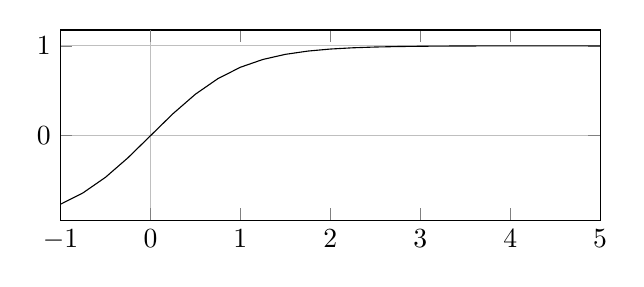
\begin{tikzpicture}
			\begin{axis}[domain=-1:5, unit vector ratio*=1 1 1,
				ytick={0,1}, enlarge x limits=false, ymajorgrids,
				xtick={-1,1,2,3,4,5},
				extra x ticks=0, extra tick style={grid=major}]
				\addplot[color=black] {tanh(x)} [mark=none, smooth];
			\end{axis}
		\end{tikzpicture}
	}
\end{figure}\noindent
The clipping of negative values to 0 in previous layers of the network allows 
greater imprecision in the penultimate layers in order to predict a 0 in the 
output adjacency matrix: rather than needing to fine tune the filters to produce 
exactly 0 for nonexistent connections, the model need only drive the values for 
such neuron pairs into the negatives, and let the application of ReLU correct.  

Similarly, the final layer \textit{tanh} allows the network to drive weights for 
probable connections far into the positives, with the activation function 
ultimately truncating to 1.

\subsection{Loss \& Optimization}
MAKE SURE YOU TALK ABOUT LOSS AND GENERAL CONCEPTS IN BG

The loss function must provide useful values to the optimizer in order to allow 
effective gradient descent towards the goal.

\subsubsection{Loss Function}
We defined a custom loss function to reflect the relative 


\subsubsection{Optimizer Function}
